\chapter{La respiración celular y la fermentación}\label{ch:g12:respiration-fermentation}

Los músculos de una corredora de maratón gastan, a lo largo de tres
horas y media, alrededor de medio mol de \omterm{def:g12:respiration-fermentation:atp}{ATP} por minuto --- un cuarto
de kilo de la molécula, fabricada, usada y rehecha miles de veces a
partir de una reserva que duraría cinco segundos. Cada una de esas
moléculas de \omterm{def:g12:respiration-fermentation:atp}{ATP} se paga con una glucosa o un ácido graso desmontados
átomo a átomo, y con una molécula de oxígeno inspirada al principio y
espirada como agua al final. El \cref{ch:g10:cell-metabolism} dio el
balance; este capítulo abre la \omterm{def:g10:cells-common-unit:organelle}{mitocondria} y sigue a la glucosa por las
tres etapas que convierten su energía en \omterm{def:g12:respiration-fermentation:atp}{ATP} --- y muestra qué hace una
\omterm{def:g10:cells-common-unit:cell}{célula} cuando se le acaba el oxígeno.

\section{El ATP, la moneda}

\begin{definition}[ATP]\label{def:g12:respiration-fermentation:atp}
El \emph{ATP}\index{ATP} (trifosfato de adenosina) es un \omterm{def:g10:universal-dna:nucleotide}{nucleótido} que
lleva tres grupos fosfato en fila. Quitar el último libera unos
\qty{30}{kJ} por mol en las condiciones de la \omterm{def:g10:cells-common-unit:cell}{célula}, y todos los
procesos de la \omterm{def:g10:cells-common-unit:cell}{célula} que exigen energía --- la contracción, el
transporte, la síntesis, la luz de una luciérnaga --- están impulsados
por esa retirada. El producto, el ADP, se recarga en ATP mediante las
reacciones de este capítulo. Una \omterm{def:g10:cells-common-unit:cell}{célula} guarda ATP para unos pocos
segundos y lo renueva de continuo; un ser humano en reposo recicla al
día alrededor de su propia masa corporal de ATP.
\end{definition}

\begin{proposition}[Dónde está la energía]\label{prop:g12:respiration-fermentation:oxidation}
La glucosa almacena energía en sus enlaces carbono--hidrógeno;
liberarla significa transferir el hidrógeno, con sus electrones, al
oxígeno --- oxidar la glucosa a dióxido de carbono y reducir el oxígeno
a agua. Hecho de un solo paso, como en una llama, la energía se iría
como calor. La \omterm{def:g10:cells-common-unit:cell}{célula} lo hace en decenas de pasos pequeños, cada uno
gobernado por una \omterm{def:g11:enzymes-and-phenotype:enzyme}{enzima}, y captura parte de la energía en varios de
ellos: el hidrógeno se carga primero en unas moléculas transportadoras
--- el \emph{NAD reducido} --- y solo al final se entrega al oxígeno.
\end{proposition}
\admitted

\section{Tres etapas}

\begin{proposition}[La glucólisis]\label{prop:g12:respiration-fermentation:glycolysis}
En el \omterm{def:g10:cells-common-unit:cell}{citoplasma}, sin oxígeno, una glucosa (seis carbonos) se parte en
dos moléculas de \emph{piruvato} (tres carbonos cada una) mediante diez
pasos enzimáticos: la \emph{glucólisis}\index{glucólisis}. El balance:
dos \omterm{def:g12:respiration-fermentation:atp}{ATP} consumidos para arrancar, cuatro producidos, o sea una ganancia
neta de 2 \omterm{def:g12:respiration-fermentation:atp}{ATP}, y dos NAD reducido cargados de hidrógeno. El piruvato
todavía guarda la mayor parte de la energía de la glucosa.
\end{proposition}
\admitted

\begin{proposition}[La mitocondria completa la oxidación]\label{prop:g12:respiration-fermentation:mitochondrion}
Cuando hay oxígeno disponible, el piruvato entra en la
\emph{mitocondria}\index{mitocondria}, un \omterm{def:g10:cells-common-unit:organelle}{orgánulo} delimitado por dos
membranas, la interna plegada en \emph{crestas} que encierran un
líquido, la \emph{matriz}.
\begin{itemize}
  \item En la matriz, cada piruvato se desmonta en un ciclo de
        reacciones, el \emph{ciclo de Krebs}\index{ciclo de Krebs}: sus
        tres carbonos salen como tres $\mathrm{CO_2}$, su hidrógeno se
        carga en los transportadores (NAD reducido y un segundo
        transportador) y se fabrica un poco de \omterm{def:g12:respiration-fermentation:atp}{ATP} directamente ---
        uno por piruvato.
  \item En la membrana interna, los transportadores cargados entregan
        sus electrones a una cadena de \omterm{def:g10:chemistry-of-life:families}{proteínas}, la \emph{cadena
        respiratoria}, que los va pasando hasta el oxígeno, que se
        combina con protones para formar agua. La energía liberada a lo
        largo de la cadena bombea protones al otro lado de la membrana,
        y su regreso a través de una \omterm{def:g11:enzymes-and-phenotype:enzyme}{enzima} rotatoria impulsa la
        síntesis de \omterm{def:g12:respiration-fermentation:atp}{ATP} --- unos 26 por glucosa.
\end{itemize}
Total para una glucosa: unos 30 \omterm{def:g12:respiration-fermentation:atp}{ATP} (2 de la \omterm{prop:g12:respiration-fermentation:glycolysis}{glucólisis}, 2 del ciclo,
unos 26 de la cadena), seis $\mathrm{CO_2}$ liberados, seis
$\mathrm{O_2}$ consumidos, y el resto de los \qty{2870}{kJ} como calor.
\end{proposition}
\begin{proof}[Pruebas experimentales]
Unas \omterm{def:g10:cells-common-unit:organelle}{mitocondrias} aisladas en una cámara cerrada con una sonda de
oxígeno no consumen oxígeno cuando se les da glucosa, pero lo consumen
deprisa cuando se les da piruvato --- la \omterm{def:g10:cells-common-unit:organelle}{mitocondria} no puede partir de
la glucosa; el \omterm{def:g10:cells-common-unit:cell}{citoplasma} tiene que hacerlo. Si se añade un veneno de
la cadena respiratoria (cianuro), el consumo se detiene de inmediato,
sea cual sea el \omterm{def:g11:enzymes-and-phenotype:enzyme}{sustrato} presente. Si se añade ADP, el consumo se
acelera, y al agotarse el ADP se frena: el uso del oxígeno está
acoplado a la síntesis de \omterm{def:g12:respiration-fermentation:atp}{ATP}. Y las \omterm{def:g10:cells-common-unit:organelle}{mitocondrias} del músculo de vuelo
de un colibrí, o del muslo de una corredora de maratón, tienen las
crestas varias veces más apretadas que las de un tejido en reposo.
\end{proof}

\begin{omfigure}
\begin{tikzpicture}
  \node[anchor=south west, inner sep=0] (img) at (0,0)
    {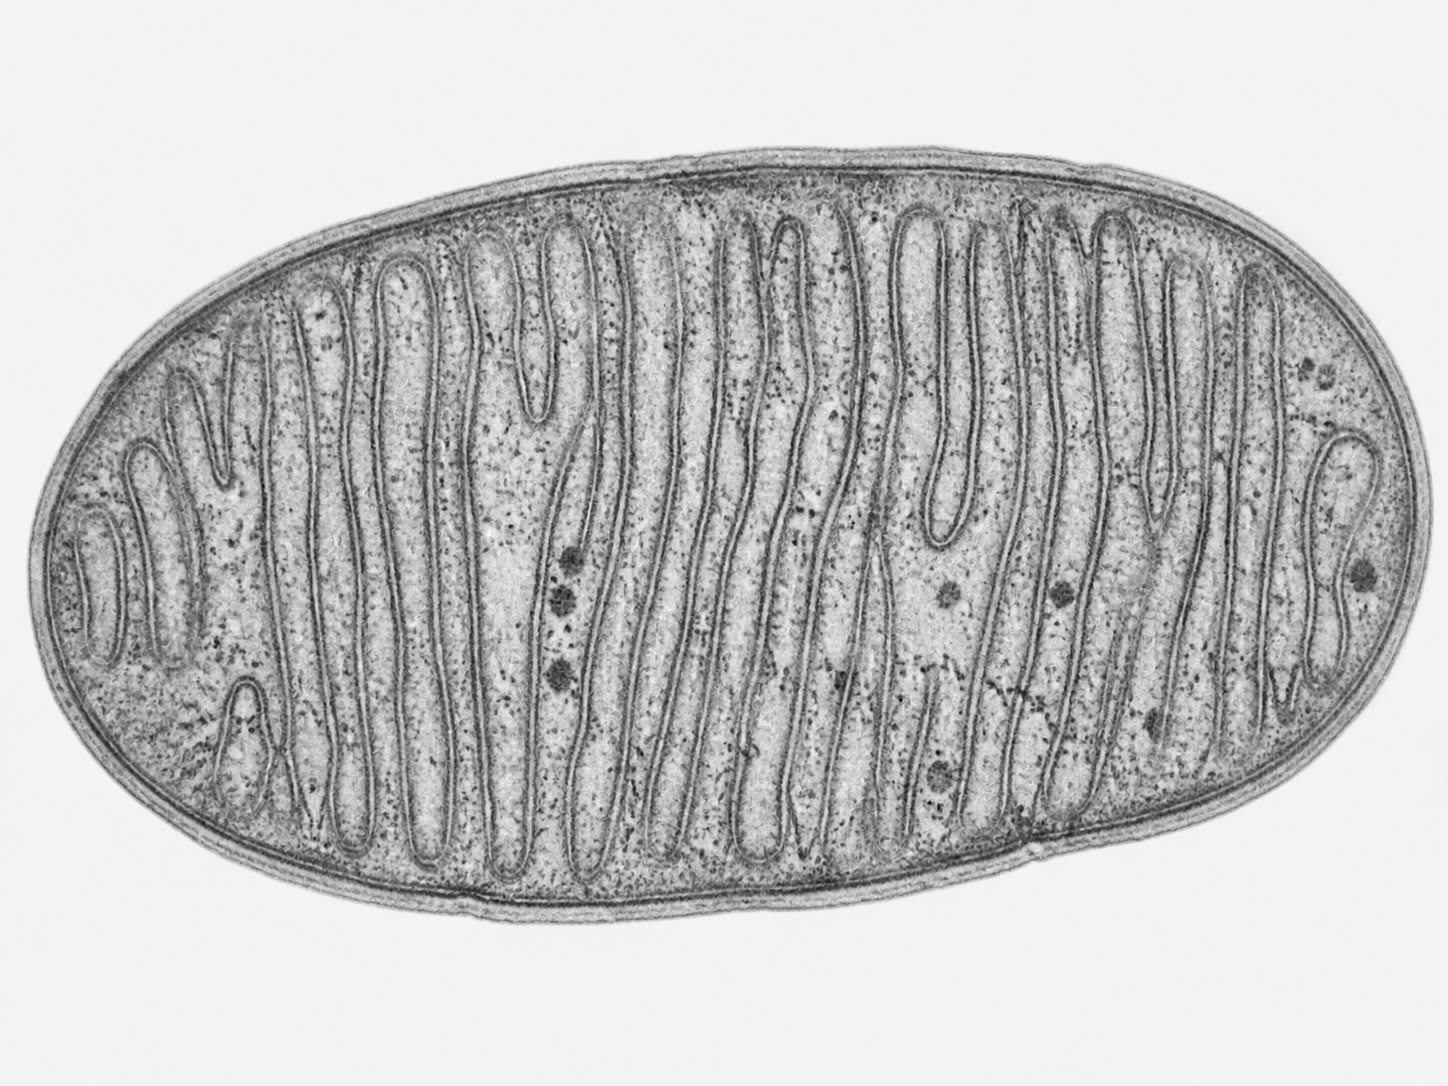
\includegraphics[width=0.5\linewidth]{images/book2/ai/g12-resp-mitochondrion-tem.jpg}};
  \begin{scope}[x={(img.south east)}, y={(img.north west)},
      every node/.style={font=\small}]
    \draw[omDef, thick] (0.08,0.55) -- (-0.04,0.80) node[left, align=right] {membrana\\ externa};
    \draw[omDef, thick] (0.20,0.45) -- (-0.04,0.25) node[left, align=right] {membrana interna,\\ plegada en crestas};
    \draw[omDef, thick] (0.55,0.50) -- (0.55,-0.06) node[below] {matriz (ciclo de Krebs)};
    \draw[omDef, thick] (0.80,0.60) -- (1.04,0.80) node[right, align=left] {crestas: la cadena\\ respiratoria};
  \end{scope}
\end{tikzpicture}

{\small Una \omterm{def:g10:cells-common-unit:organelle}{mitocondria} en el microscopio electrónico. La membrana
interna está plegada en crestas, que llevan la cadena respiratoria y la
\omterm{def:g11:enzymes-and-phenotype:enzyme}{enzima} que fabrica \omterm{def:g12:respiration-fermentation:atp}{ATP}; el líquido que hay entre ellas, la matriz,
ejecuta el \omterm{prop:g12:respiration-fermentation:mitochondrion}{ciclo de Krebs}.}
\end{omfigure}

\begin{omfigure}
\begin{tikzpicture}[font=\small, >=Stealth,
  b/.style={draw, rounded corners, align=center, minimum height=0.9cm}]
  % cytoplasm region
  \node[b, fill=omDef!8, minimum width=6.0cm, minimum height=6.2cm] (cyt) at (0,0) {};
  \node[anchor=north, font=\small\bfseries] at (cyt.north) {citoplasma};
  \node[b, fill=omMeth!20, text width=2.4cm] (glu) at (0,2.0) {glucosa (6 C)};
  \node[b, fill=omProp!20, text width=2.4cm] (pyr) at (0,-0.2) {2 piruvatos\\ (3 C cada uno)};
  \draw[->, thick] (glu) -- node[right, align=left, font=\scriptsize] {glucólisis:\\ $+2$ ATP, $+2$ NADH} (pyr);
  \node[b, fill=omThm!15, text width=2.6cm] (ferm) at (0,-2.4) {fermentación:\\ lactato, o bien\\ etanol $+ \mathrm{CO_2}$};
  \draw[->, thick, omThm] (pyr) -- node[right, font=\scriptsize, align=left] {sin $\mathrm{O_2}$:\\ el NADH se regenera} (ferm);
  % mitochondrion region
  \node[b, fill=omProp!8, minimum width=6.4cm, minimum height=6.2cm, rounded corners=14pt] (mit) at (7.3,0) {};
  \node[anchor=north, font=\small\bfseries] at (mit.north) {mitocondria};
  \node[b, fill=omProp!20, text width=2.6cm] (krebs) at (7.3,1.4) {ciclo de Krebs\\ (matriz):\\ salen $6\,\mathrm{CO_2}$,\\ $+2$ ATP, transportadores cargados};
  \node[b, fill=omThm!15, text width=2.8cm] (chain) at (7.3,-1.5) {cadena respiratoria\\ (membrana interna):\\ transportadores $+ \mathrm{O_2} \to \mathrm{H_2O}$,\\ $+26$ ATP};
  \draw[->, thick] (pyr.east) -- node[pos=0.72, above, font=\scriptsize] {con $\mathrm{O_2}$} (krebs.west |- pyr.east);
  \draw[->, thick] (krebs) -- node[right, font=\scriptsize] {NAD reducido} (chain);
  \draw[->, thick] (10.9,-1.1) -- (chain.east |- 0,-1.1) node[pos=0, right] {$6\,\mathrm{O_2}$};
  \draw[->, thick] (chain.east |- 0,-1.9) -- (10.9,-1.9) node[right] {$6\,\mathrm{H_2O}$};
  \draw[->, thick] (krebs.east |- 0,1.8) -- (10.9,1.8) node[right] {$6\,\mathrm{CO_2}$};
\end{tikzpicture}

{\small Las tres etapas de la respiración, y el atajo de la
\omterm{def:g10:cell-metabolism:fermentation}{fermentación}. La \omterm{prop:g12:respiration-fermentation:glycolysis}{glucólisis}, en el \omterm{def:g10:cells-common-unit:cell}{citoplasma}, rinde dos \omterm{def:g12:respiration-fermentation:atp}{ATP} y dos
piruvatos; en la \omterm{def:g10:cells-common-unit:organelle}{mitocondria}, el \omterm{prop:g12:respiration-fermentation:mitochondrion}{ciclo de Krebs} los reduce a dióxido de
carbono y carga los transportadores, que la cadena respiratoria
descarga sobre el oxígeno mientras fabrica la mayor parte del \omterm{def:g12:respiration-fermentation:atp}{ATP}. Sin
oxígeno, el piruvato se desvía a la \omterm{def:g10:cell-metabolism:fermentation}{fermentación}, que no rinde nada
más.}
\end{omfigure}

\begin{example}[Leer un registro de oxígeno]\label{ex:g12:respiration-fermentation:trace}
Unas \omterm{def:g10:cells-common-unit:organelle}{mitocondrias} aisladas en la cámara: el oxígeno se queda en
\qty{8}{mg/L}; se añade glucosa, nada; se añade piruvato, el oxígeno
baja a \qty{0.5}{mg/L} por minuto; se añade ADP, la bajada se hace más
pronunciada, \qty{1.5}{mg/L} por minuto durante un rato, y vuelve
después a \num{0.5}; se añade cianuro, la bajada se detiene. Cuatro
hechos en un solo registro: la \omterm{def:g10:cells-common-unit:organelle}{mitocondria} necesita piruvato, no
glucosa; el uso del oxígeno está acoplado a la síntesis de \omterm{def:g12:respiration-fermentation:atp}{ATP}; el
acoplamiento pasa por la cadena que el cianuro bloquea; y una
\omterm{def:g10:cells-common-unit:organelle}{mitocondria} sin trabajo que hacer marcha al ralentí.
\end{example}

\begin{omfigure}
\begin{tikzpicture}
\begin{axis}[
  width=0.9\linewidth, height=5.6cm,
  axis x line=bottom, axis y line=left,
  xmin=0, xmax=16, ymin=0, ymax=10,
  xlabel={tiempo (min)}, ylabel={$\mathrm{O_2}$ disuelto (mg/L)},
  xlabel style={font=\small, at={(axis description cs:0.5,-0.12)}, anchor=north},
  ylabel style={font=\small},
  tick label style={font=\small}, xtick={0,2,4,6,8,10,12,14,16}, ytick={0,2,4,6,8},
  clip=false,
]
\addplot[thick, omThm] coordinates {(0,8) (2,8) (4,8) (6,7) (8,4) (10,3) (12,2) (14,2) (16,2)};
\draw[->, thick] (axis cs:2,9.6) -- (axis cs:2,8.4);
\node[font=\scriptsize, anchor=south] at (axis cs:2,9.7) {glucosa};
\draw[->, thick] (axis cs:4,9.6) -- (axis cs:4,8.4);
\node[font=\scriptsize, anchor=south] at (axis cs:4,9.7) {piruvato};
\draw[->, thick] (axis cs:6,9.6) -- (axis cs:6,8.4);
\node[font=\scriptsize, anchor=south] at (axis cs:6,9.7) {ADP};
\draw[->, thick] (axis cs:12,9.6) -- (axis cs:12,8.4);
\node[font=\scriptsize, anchor=south] at (axis cs:12,9.7) {cianuro};
\end{axis}
\end{tikzpicture}

{\small Consumo de oxígeno de unas \omterm{def:g10:cells-common-unit:organelle}{mitocondrias} aisladas. La glucosa no
hace nada; el piruvato pone en marcha el consumo; el ADP lo acelera
hasta que se gasta; el cianuro, que bloquea la cadena respiratoria, lo
detiene.}
\end{omfigure}

\section{Sin oxígeno: la fermentación}

\begin{proposition}[La fermentación regenera el transportador]\label{prop:g12:respiration-fermentation:fermentation}
La \omterm{prop:g12:respiration-fermentation:glycolysis}{glucólisis} carga dos transportadores NAD por glucosa; con oxígeno,
la \omterm{def:g10:cells-common-unit:organelle}{mitocondria} los descarga. Sin oxígeno, todos los transportadores
estarían cargados en unos segundos y la \omterm{prop:g12:respiration-fermentation:glycolysis}{glucólisis} se pararía. La
\emph{fermentación}\index{fermentación} es la manera que tiene el
\omterm{def:g10:cells-common-unit:cell}{citoplasma} de descargarlos: el propio piruvato acepta el hidrógeno y se
convierte en \emph{lactato} (\omterm{def:g10:cells-common-unit:cell}{células} musculares, bacterias de la leche)
o, tras perder un $\mathrm{CO_2}$, en \emph{etanol} (levadura). No se
fabrica más \omterm{def:g12:respiration-fermentation:atp}{ATP}; el rendimiento son los 2 \omterm{def:g12:respiration-fermentation:atp}{ATP} de la \omterm{prop:g12:respiration-fermentation:glycolysis}{glucólisis}, unas
quince veces menos que el de la respiración, y el producto --- lactato
o etanol --- todavía guarda la mayor parte de la energía de la glucosa.
\end{proposition}
\admitted

\begin{omfigure}
\begin{tikzpicture}
\begin{axis}[
  ybar, bar width=22pt,
  width=0.7\linewidth, height=5.2cm,
  axis x line=bottom, axis y line=left,
  ymin=0, ymax=36, ylabel={ATP por glucosa},
  ylabel style={font=\small},
  symbolic x coords={fermentación, glucólisis + Krebs, respiración completa},
  xtick=data, tick label style={font=\small},
  enlarge x limits=0.3, ytick={0,10,20,30},
  nodes near coords, nodes near coords style={font=\small},
]
\addplot[fill=omThm!45, draw=omThm] coordinates {(fermentación,2) (glucólisis + Krebs,4) (respiración completa,30)};
\end{axis}
\end{tikzpicture}

{\small Rendimiento en \omterm{def:g12:respiration-fermentation:atp}{ATP} por glucosa. La \omterm{prop:g12:respiration-fermentation:glycolysis}{glucólisis} sola, con la
\omterm{def:g10:cell-metabolism:fermentation}{fermentación} para regenerar su transportador, da 2; el \omterm{prop:g12:respiration-fermentation:mitochondrion}{ciclo de Krebs}
añade 2 directamente; la cadena respiratoria, que necesita oxígeno,
añade los otros 26.}
\end{omfigure}

\begin{example}[La elección del músculo]\label{ex:g12:respiration-fermentation:muscle}
Una fibra muscular de velocista necesita \omterm{def:g12:respiration-fermentation:atp}{ATP} más deprisa de lo que
pueden fabricarlo sus \omterm{def:g10:cells-common-unit:organelle}{mitocondrias} y su suministro de oxígeno; la
\omterm{prop:g12:respiration-fermentation:glycolysis}{glucólisis} con \omterm{def:g10:cell-metabolism:fermentation}{fermentación} láctica entrega \omterm{def:g12:respiration-fermentation:atp}{ATP} tres veces más deprisa,
a quince veces el coste en glucosa, y el lactato se acumula hasta que
el dolor detiene el esfuerzo. Las fibras de una corredora de maratón
funcionan con la respiración, despacio y casi indefinidamente, y queman
grasa además de glucosa; sus \omterm{def:g10:cells-common-unit:organelle}{mitocondrias} son más grandes y más
numerosas, sus capilares más densos, y su lactato se mantiene bajo. Los
tipos de fibra del \cref{ch:g10:muscles-and-joints} son estas dos
estrategias construidas dentro de las \omterm{def:g10:cells-common-unit:cell}{células}.
\end{example}

\begin{method}[Cuadrar un presupuesto de energía]\label{met:g12:respiration-fermentation:budget}
\begin{enumerate}
  \item Convierte la potencia necesaria en \omterm{def:g12:respiration-fermentation:atp}{ATP}: a unos \qty{30}{kJ}
        aprovechables por mol de \omterm{def:g12:respiration-fermentation:atp}{ATP}, \qty{1}{kW} de potencia
        metabólica son \qty{2}{mol} de \omterm{def:g12:respiration-fermentation:atp}{ATP} por minuto.
  \item Convierte el \omterm{def:g12:respiration-fermentation:atp}{ATP} en combustible: 30 \omterm{def:g12:respiration-fermentation:atp}{ATP} por glucosa en la
        respiración, 2 en la \omterm{def:g10:cell-metabolism:fermentation}{fermentación}.
  \item Convierte el combustible en oxígeno: 6 $\mathrm{O_2}$ por
        glucosa respirada, \qty{24}{L} por mol de gas.
  \item Compara el oxígeno necesario con el que entrega la sangre
        (\cref{ch:g10:heart-lungs-effort}): el déficit lo cubre la
        \omterm{def:g10:cell-metabolism:fermentation}{fermentación}, con su lactato.
\end{enumerate}
\end{method}

\begin{remark}[El espejo de la fotosíntesis]\label{rem:g12:respiration-fermentation:mirror}
La \omterm{def:g10:cell-metabolism:autotrophy}{fotosíntesis} carga con luz los electrones del agua en unos
transportadores y los usa para reducir el dióxido de carbono a azúcar,
con liberación de oxígeno; la respiración descarga los electrones del
azúcar en unos transportadores y se los pasa al oxígeno, con lo que
forma agua y libera dióxido de carbono, y usa la energía para fabricar
\omterm{def:g12:respiration-fermentation:atp}{ATP}. Las dos las ejecutan unos \omterm{def:g10:cells-common-unit:organelle}{orgánulos} que fueron ambos, en su día,
bacterias libres (\cref{ch:g12:diversification-of-life}), y el
\omterm{def:g12:photosynthesis:chloroplast}{cloroplasto} suministra lo que la \omterm{def:g10:cells-common-unit:organelle}{mitocondria} consume; entre las dos
convierten la luz del sol en la moneda de todas las \omterm{def:g10:cells-common-unit:cell}{células}, y el
oxígeno de la atmósfera es el saldo de sus cuentas.
\end{remark}

\section{Ejercicios}

\begin{exercise}[$\star$]\label{exo:g12:respiration-fermentation:1}
¿Qué es el \omterm{def:g12:respiration-fermentation:atp}{ATP}, y qué pasa cuando una \omterm{def:g10:cells-common-unit:cell}{célula} lo usa?
\end{exercise}

\begin{exercise}[$\star$]\label{exo:g12:respiration-fermentation:2}
Nombra las tres etapas de la respiración, di dónde ocurre cada una y
qué rinde cada una.
\end{exercise}

\begin{exercise}[$\star$]\label{exo:g12:respiration-fermentation:3}
Describe la \omterm{def:g10:cells-common-unit:organelle}{mitocondria} y di qué etapa se desarrolla en cada uno de sus
compartimentos.
\end{exercise}

\begin{exercise}[$\star$]\label{exo:g12:respiration-fermentation:4}
¿Qué consigue la \omterm{def:g10:cell-metabolism:fermentation}{fermentación} para la \omterm{def:g10:cells-common-unit:cell}{célula}, y qué rinde?
\end{exercise}

\begin{exercise}[$\star$]\label{exo:g12:respiration-fermentation:5}
Compara el rendimiento en \omterm{def:g12:respiration-fermentation:atp}{ATP} de la respiración y de la \omterm{def:g10:cell-metabolism:fermentation}{fermentación}, y
los productos que quedan al final de cada una.
\end{exercise}

\begin{exercise}[$\star\star$]\label{exo:g12:respiration-fermentation:6}
En el registro de oxígeno, ¿qué muestra cada una de las cuatro
adiciones?
\end{exercise}

\begin{exercise}[$\star\star$]\label{exo:g12:respiration-fermentation:7}
¿Por qué unas \omterm{def:g10:cells-common-unit:organelle}{mitocondrias} aisladas no pueden usar glucosa, mientras
que una \omterm{def:g10:cells-common-unit:cell}{célula} entera sí?
\end{exercise}

\begin{exercise}[$\star\star$]\label{exo:g12:respiration-fermentation:8}
Explica por qué la \omterm{prop:g12:respiration-fermentation:glycolysis}{glucólisis} se pararía en unos segundos sin oxígeno
si la \omterm{def:g10:cell-metabolism:fermentation}{fermentación} no existiera.
\end{exercise}

\begin{exercise}[$\star\star$]\label{exo:g12:respiration-fermentation:9}
Una \omterm{def:g10:cells-common-unit:cell}{célula} necesita 60 \omterm{def:g12:respiration-fermentation:atp}{ATP} por segundo. ¿Cuántas moléculas de glucosa
por segundo le cuesta eso por respiración, y por \omterm{def:g10:cell-metabolism:fermentation}{fermentación}?
\end{exercise}

\begin{exercise}[$\star\star$]\label{exo:g12:respiration-fermentation:10}
El cianuro es letal en unos minutos. Explica por qué, a partir de la
cadena respiratoria, y por qué fallan primero el cerebro y el corazón.
\end{exercise}

\begin{exercise}[$\star\star$]\label{exo:g12:respiration-fermentation:11}
¿De dónde viene el dióxido de carbono que espiras, etapa por etapa? ¿Y
el agua que fabrica la respiración?
\end{exercise}

\begin{exercise}[$\star\star\star$]\label{exo:g12:respiration-fermentation:12}
Un músculo produce lactato durante una carrera y, después, el hígado
vuelve a convertir el lactato en glucosa gastando \omterm{def:g12:respiration-fermentation:atp}{ATP} de la
respiración. Explica por qué el organismo entero acaba pagando más de
30 \omterm{def:g12:respiration-fermentation:atp}{ATP} por la glucosa que el músculo fermentó.
\end{exercise}

\begin{exercise}[$\star\star\star$]\label{exo:g12:respiration-fermentation:13}
Una levadura con aire usa la glucosa despacio y no fabrica etanol;
encerrada, la usa deprisa y fabrica etanol. Explícalo con los
rendimientos, y di por qué la masa del pan sube tenga o no tenga aire
la levadura.
\end{exercise}

\begin{exercise}[$\star\star\star$]\label{exo:g12:respiration-fermentation:14}
Las \omterm{def:g10:cells-common-unit:cell}{células} de la grasa parda de un recién nacido contienen
\omterm{def:g10:cells-common-unit:organelle}{mitocondrias} cuya cadena funciona sin fabricar \omterm{def:g12:respiration-fermentation:atp}{ATP}: el flujo de
protones está cortocircuitado. ¿Qué producen esas \omterm{def:g10:cells-common-unit:cell}{células} en su lugar,
y por qué le resulta útil a un recién nacido?
\end{exercise}

\begin{exercise}[$\star\star\star$]\label{exo:g12:respiration-fermentation:15}
Compara punto por punto la respiración y la \omterm{def:g10:cell-metabolism:autotrophy}{fotosíntesis}: origen y
destino de los electrones, gas consumido y gas liberado, energía que
entra y energía que sale, \omterm{def:g10:cells-common-unit:organelle}{orgánulo}. Después di en una frase por qué
ninguna de las dos puede existir en la Tierra sin la otra.
\end{exercise}

\section{Problema: Medio mol de ATP por minuto}

\begin{problem}[{Problema de fin de semana --- la energía de una
corredora seguida del vatio a la molécula: ATP contado, glucosa y
oxígeno calculados, medida la parte de las mitocondrias y el esprint
que la cadena no puede pagar}]
\label{pb:g12:respiration-fermentation:1}
Una corredora sostiene una potencia metabólica de \qty{1000}{W}, de la
que alrededor de un tercio se captura como \omterm{def:g12:respiration-fermentation:atp}{ATP} y el resto se va como
calor. Toma \qty{30}{kJ} de energía aprovechable por mol de \omterm{def:g12:respiration-fermentation:atp}{ATP}, 30 \omterm{def:g12:respiration-fermentation:atp}{ATP}
por glucosa en la respiración y 2 en la \omterm{def:g10:cell-metabolism:fermentation}{fermentación}, \qty{2870}{kJ}
por mol de glucosa, \qty{24}{L} por mol de gas y la glucosa a
\qty{180}{g/mol}.

\medskip
\noindent\textbf{Parte I --- El \omterm{def:g12:respiration-fermentation:atp}{ATP}.}
\begin{enumerate}
  \item ¿Cuántos moles de \omterm{def:g12:respiration-fermentation:atp}{ATP} usa la corredora por minuto? (Solo cuenta
        el tercio capturado como \omterm{def:g12:respiration-fermentation:atp}{ATP}.)
  \item ¿Qué masa de \omterm{def:g12:respiration-fermentation:atp}{ATP} es eso, a \qty{507}{g/mol}? Compárala con los
        pocos gramos que los músculos guardan en cada momento.
  \item ¿Cuántas veces por minuto se recarga cada molécula de \omterm{def:g12:respiration-fermentation:atp}{ATP}, si
        la reserva del organismo es de \qty{50}{g}?
  \item Si ese \omterm{def:g12:respiration-fermentation:atp}{ATP} se fabricara solo por respiración, ¿cuántos moles de
        glucosa se consumirían por minuto?
  \item ¿Cuántos litros de oxígeno por minuto exige eso? Compáralo con
        un $\dot V\!\mathrm{O_2}$máx de \qty{4}{L/min}.
\end{enumerate}

\medskip
\noindent\textbf{Parte II --- La parte de las \omterm{def:g10:cells-common-unit:organelle}{mitocondrias}.}
\begin{enumerate}[resume]
  \item De los 30 \omterm{def:g12:respiration-fermentation:atp}{ATP} por glucosa, ¿cuántos se fabrican en el
        \omterm{def:g10:cells-common-unit:cell}{citoplasma} y cuántos en la \omterm{def:g10:cells-common-unit:organelle}{mitocondria}? ¿Qué fracción del \omterm{def:g12:respiration-fermentation:atp}{ATP}
        de la corredora es mitocondrial?
  \item ¿Cuántos moles de $\mathrm{CO_2}$ espira por minuto, y de qué
        etapa de la respiración vienen?
  \item ¿Cuánto de los \qty{2870}{kJ} de una glucosa acaba en \omterm{def:g12:respiration-fermentation:atp}{ATP}?
        ¿Adónde va el resto, y qué hace la corredora al respecto?
  \item Las \omterm{def:g10:cells-common-unit:organelle}{mitocondrias} de sus músculos tienen una superficie total de
        membrana interna de unos \qty{1000}{m^2}. ¿Por qué necesita
        tanta superficie la cadena?
  \item El \omterm{def:g10:sport-and-health:training}{entrenamiento} duplica las \omterm{def:g10:cells-common-unit:organelle}{mitocondrias} de sus fibras. ¿Qué
        cantidades de las anteriores cambia eso, y cuáles no?
\end{enumerate}

\medskip
\noindent\textbf{Parte III --- El esprint.}
En el esprint final, sus músculos necesitan \qty{800}{W} de potencia en
forma de \omterm{def:g12:respiration-fermentation:atp}{ATP} durante 30 segundos, mientras que la respiración, limitada
por el oxígeno que entrega la sangre, puede suministrar como mucho
\qty{400}{W} en forma de \omterm{def:g12:respiration-fermentation:atp}{ATP}.
\begin{enumerate}[resume]
  \item ¿Cuántos moles de \omterm{def:g12:respiration-fermentation:atp}{ATP} exige el esprint en total?
  \item ¿Cuánto de ellos puede suministrar la respiración en 30
        segundos, y cuánto tiene que venir de la \omterm{def:g10:cell-metabolism:fermentation}{fermentación}?
  \item ¿Cuántos moles de glucosa consume la parte fermentada, y
        cuántos moles de lactato deja?
  \item Compara la glucosa gastada por \omterm{def:g12:respiration-fermentation:atp}{ATP} en las dos vías durante el
        esprint. ¿Por qué acepta el músculo el derroche?
  \item Después de la carrera, el lactato se oxida o se vuelve a
        convertir en glucosa. Explica por qué su consumo de oxígeno
        sigue alto durante varios minutos después de pararse.
\end{enumerate}

\medskip
\noindent\textbf{Parte IV --- El otro combustible.}
La grasa suministra unos \qty{38}{kJ} por gramo y, por gramo, necesita
alrededor de un 20\% más de oxígeno que la glucosa para la misma
energía.
\begin{enumerate}[resume]
  \item Si la mitad de sus \qty{1000}{W} viniera de la grasa, ¿qué masa
        de grasa quemaría por hora?
  \item ¿Por qué la grasa, aunque es más rica en energía por gramo, da
        menos potencia por litro de oxígeno?
  \item Los ácidos grasos entran en la respiración por el \omterm{prop:g12:respiration-fermentation:mitochondrion}{ciclo de
        Krebs} y se saltan la \omterm{prop:g12:respiration-fermentation:glycolysis}{glucólisis}. ¿Cuál de las tres etapas no
        puede usar entonces la grasa, y qué se sigue de ello para un
        esprint?
  \item ¿Por qué el cerebro, que funciona solo con glucosa, sigue
        trabajando durante la carrera aunque los músculos se estén
        llevando casi toda la glucosa de la sangre?
  \item Enuncia el resultado: los moles de \omterm{def:g12:respiration-fermentation:atp}{ATP} que usa la corredora por
        minuto, los litros de oxígeno que los pagan y la etapa de la
        respiración que fabrica la mayoría de ellos.
\end{enumerate}
\end{problem}
